\chapter{基于图模型的方面级情感分析算法}
第三章探讨了基于图模型理论的整体文本分类算法,图模型应用于文本分类任务取得了一定效果。尤其是考虑作为全局信息而引入的超节点
对模型性能有一定的正面影响。超节点实际上不仅仅可以作为全局信息而使用,根据不同任务可以设置不同类型的超节点。本章依旧基于图模型
理论,探讨关于方面级情感分析的任务。本章算法超节点不再使用全局信息而使用方面词信息,并与第三章构图方式一致,建立文本图结构,实现方面级
情感分析。

\section{引言}
方面级情感分类\citing{zhou2019deep}已经越来越备受关注,相比于一般的文本分类算法具有更高的实用性。例如对于在美团、京东、天猫等平台上进行的商品评价描述,
采用方面级的情感分类可以针对商品不同的方面进行评价,进而实现对产品全方位的点评,并且平台可以根据点评的方面以于分类,以保障用户对不同方面的感知和需求。
比如有些用户看重服务,有些用户看重质量。同时商家可以根据用户对不同方面的评价进行改进,提升商品整体质量。方面级情感分类相比于一般的文本分类算法,具有一定难度。

Li等人\citing{li2018transformation}使用一个Bi-LSTM模型处理文本序列,获取每个单词的中间隐藏状态的向量表示,随后每个单词向量对应一个CPT结构(Context-Preserving Transformation)。
每个CPT中采用Bi-LSTM模型学习一个方面词对应的信息向量然后与输入的单词向量拼接获取一个新的单词向量,该向量体现了每个单词与目标词之间的关系信息。
通过CPT层后,每个单词具有一个新的向量表示,再对这组向量表示采用CNN模型卷积处理,捕捉关键信息,生成表示文本的向量,用以实现分类。
Wang等人\citing{wang2016attention}提出了一个基于LSTM的注意力机制模型。它将方面词的向量表示分别与文本内容的每个单词向量表示进行拼接,组合成新的向量,作为LSTM模型的输入。
随后将LSTM模型获得的每步单词的隐藏状态与方面词向量用一个注意力机制求得权重,代表了每个单词对目标情感的贡献度。最后通过向量加权和表示最终的用以分类的向量表示。虽然
这些方法取得了一定效果,但是使用不能并行计算的LSTM模型,计算效率相对较低。同时方面级的目标词与文本内容单词之间应该存在许多联系,
如果能够挖掘它们之间的内在关系,便能进一步学到情感信息。

本章基于第三章提出的图模型算法,进一步改进使之适合方面级情感分析任务。具体来说,本章的算法不再使用依据语料库信息构建超节点,而是使用对应的方面词构建,即希望这个超节点学习到的
是方面词信息,同时将这个信息通过图结构传递给其他单词节点。文本图其他部分构建过程采用第三章描述的方式一致。考虑到门控机制具有选择遗忘的功能,而图卷积神经网络
每一层的节点信息对于下一层并不一定都有用,因此,本章采用一个门控机制去控制每层节点信息的流动。通过图模型学习,将获得每个单词新的向量表示以及一个表示为方面词的信息向量。
方面词的具体情感信息取决于文本中对应位置的情感词汇,因此,本章继续采用一个注意力机制,通过方面词向量去查询所有单词中对它情感偏向最重要的词汇,获得相应的权重,最后将这些向量进行
加权和,得到最终的用以实现分类任务的向量。

综上所示,本章提出的方法主要有以下三点特色:\noindent\textcircled{1}采用一个超节点表示方面词信息,并将这个信息通过图网络进行传递,进而捕捉文本单词以及方面词之间的关系,学到两者的向量表示。
\noindent\textcircled{2}通过门控机制选择或遗忘传递给图模型中下一层的信息。\noindent\textcircled{3}利用注意力机制寻找对目标词情感贡献最大的词汇。

\section{问题定义}
本章主要探讨的是方面级情感分类任务。对于这类任务不同于整体文本分类任务,每个文本中都有一个或多个方面词。如句子“great food but the service was dreadful”,这个句子中定义
了两个方面词一个是“food”,另一个是“service”,方面级情感分类任务的目标就是判断这两个方面词对应的情感倾向。如“food”这个词,采用“great”进行形容,是一个褒义词,因此对于“food”的情感
可以归属于正向的。而对于“service”这个词,是使用“dreadful”进行描述的,属于贬义词,因此情感归属于负面。

某一文本数据$T_i$由一组$n$个单词以及多个方面词构成,$T_i=[w_1,a_{i}...a_{j},w_{n-1},w_n]$。其中$w$表示一个单词,$a_i$表示为第$i$个方面词,通常方面词由一个或多个单词组成。
文本中每个单词都有一个对应的单词向量,本章采用的单词向量主要是从Glove或经过BERT模型后得到。因此一个文本可以由一个$\mathbb{R}^{n\times d}$的向量矩阵表示,其中$n$
表示文本中单词的个数,$d$表示为单词向量的维度。方面级情感分类任务就是学得一个函数$F(\cdot)$,输入这段文本以及需要分析的这段文本中的方面词,输出这个方面词对应的情感倾向,即判断
这个方面词是正向的或是负面的或是无情感。

\section{算法模型设计}
以前的一些研究仅仅直接对方面词的向量以及文本向量进行拼接,并未细致考虑方面词与文本中其他单词之间的联系。如果能够挖掘它们之间的内在关系,便能进一步提升模型性能。此外在图卷积网络计算中
,网络层数的增加意味着当前节点将会获取得到更远处节点的信息。而更远处节点的信息不一定对当前节点有用,因此本章采用一个门控机制,选择性的选择或是遗忘节点信息,控制信息流动,进一步提升模型
性能,确保学到更有效的向量表示。注意力机制使得模型关注于重要信息,查找对于方面词情感分析更为重要的词汇。本节主要详细阐述了算法模型,首先介绍了模型的整体设计,之后再详细介绍
每一步的具体实现。

\subsection{模型总览}
本章实现的方面级情感分析算法流程图如图\ref{asgraphLct}所示。预处理是指对文本数据进行统一的规则化处理,首先将所有文本都处理成小写字体,同时删除部分无关的词汇,比如一些停止词等。
建立词汇表,不同的单词应该对应一个唯一的索引,有助于后期处理时正确找到每个单词所对应的嵌入向量。同时需要标注每个文本中对应的方面词所在位置,便于后续分析任务使用。
\begin{figure}[htb]
	\setlength{\belowcaptionskip}{0pt}
	\centering
	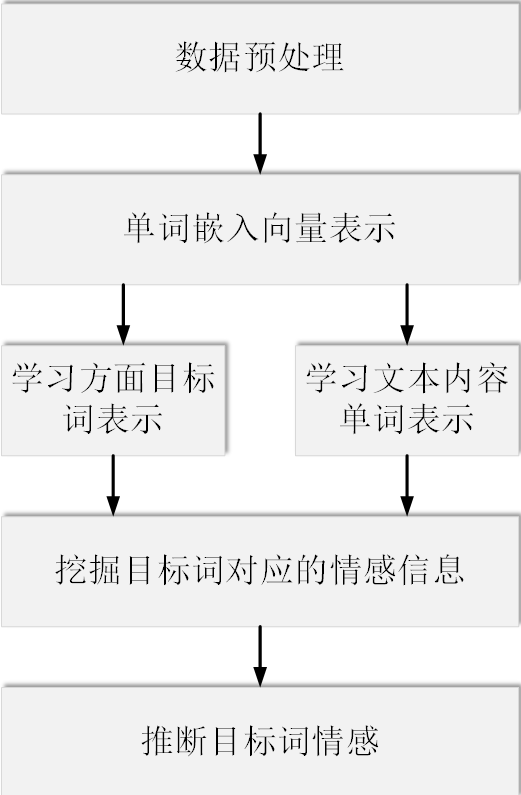
\includegraphics[width=0.3\textwidth]{pic/asgraph.png}
	\caption{方面级情感分析算法流程图}
	\label{asgraphLct}
\end{figure}
方面词向量以及文本单词向量的学习都是基于图网络模型,经过图卷积神经网络学得到一个超节点向量,即表示为方面词向量,以及每个单词的新的向量表示。方面词关键词汇信息挖掘即是使用注意力机制
关注重点词汇,找出对该方面词的情感倾向有帮助的词汇,最后实现分析。

本章提出的方法是一个端到端的深度学习模型,即输入文本内容和对应的方面词,就可得到该方面词对应的情感类别。该算法总共有三个部分,如图\ref{asgraphart}所示,第一部分定义为文本构图部分,
该步骤主要是将文本中的单词采用第三章提到的构图方法构建成图,其次构造一个传递方面词信息的超节点。第二部分主要是单词词向量表示学习以及超节点的表示学习,这部分采用基于多头注意力机制的GCN
进行学习以及一个门控机制用以控制图网络模型中每一层信息的传递。第三部分是基于第二部分学到的文本词向量以及超节点向量来计算。将超节点向量作为注意力机制中的Query向量,
计算文本单词中所有单词的权重,权重的大小即可视作这个单词对方面词情感的分析的重要程度。随后将注意力机制获得向量与超节点向量进行一个简单地结合,即得到最终的分类向量,将这个向量输入一个简单的
神经网络通过softmax激活函数实现情感分析任务。以下几节将对这些部分进行详细介绍。
\begin{figure}[htb]
	\setlength{\belowcaptionskip}{0pt}
	\centering
	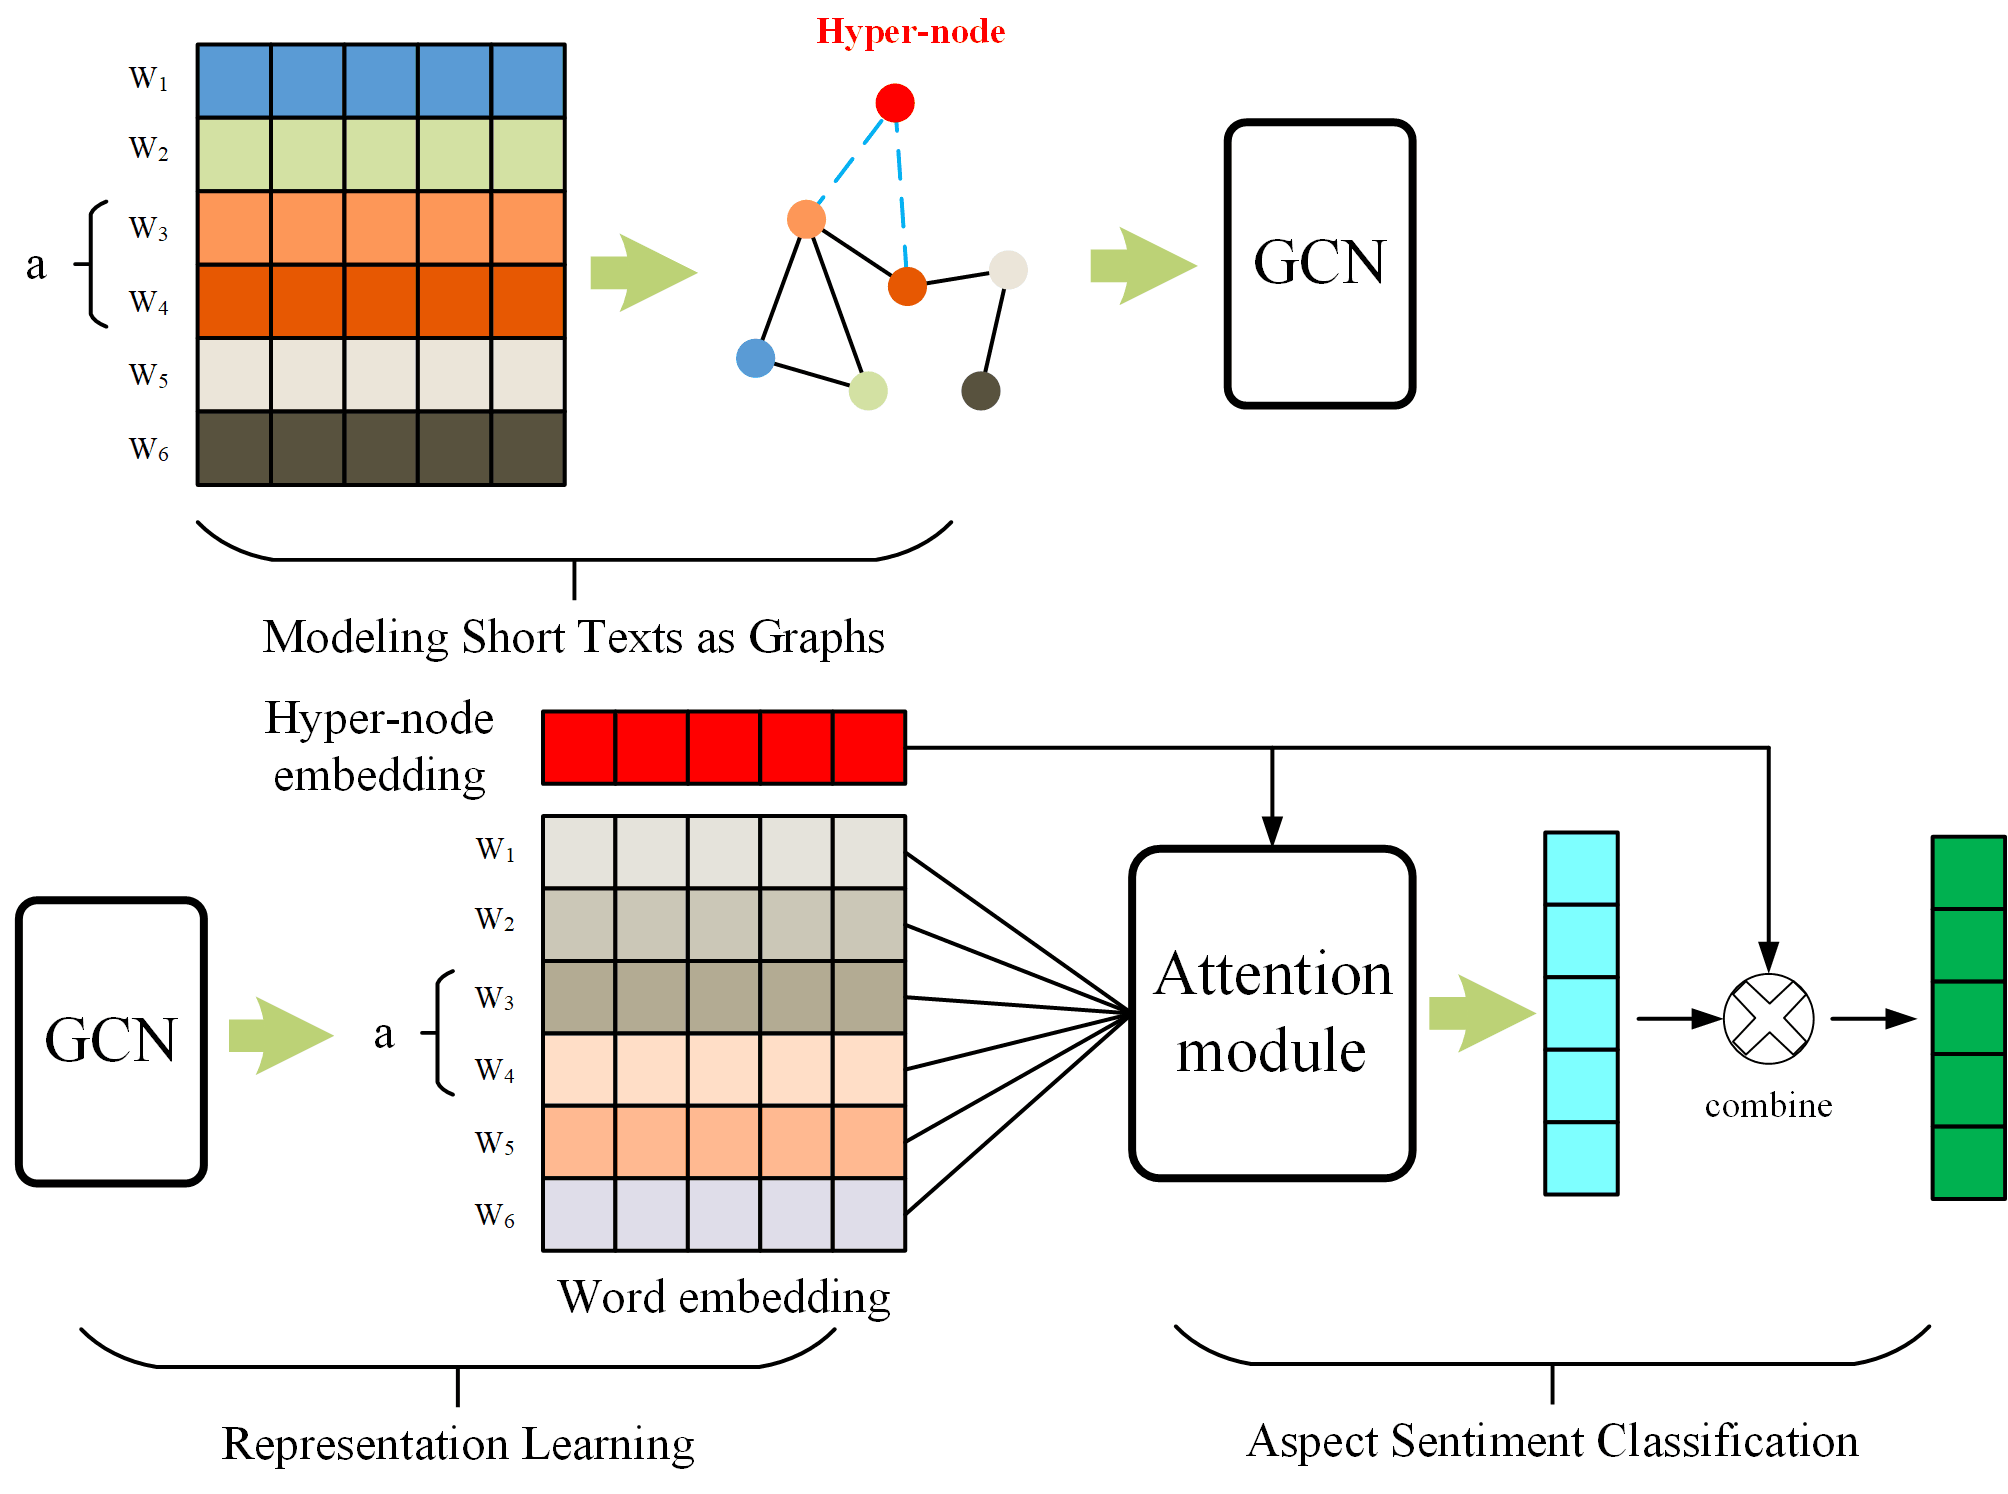
\includegraphics[width=1\textwidth]{pic/asgraphart.png}
	\caption{方面级情感分析算法模型}
	\label{asgraphart}
\end{figure}

\subsection{文本图建模过程}
本章文本图的构建过程与第三章图构建过程一致,均是采用滑动窗口的方式构建单词与单词之间的图。但与第三章略有不同,第三章中每个单词在图中仅有一个节点,即使一个单词在同一个文本中只出现了一次,
也仅仅视作一个节点。而本章中因为同时还要采用BERT预训练模型,因此构图过程中,为文本中每一个单词都构建一个节点,即使是同一个单词只要出现的位置不同,均构建一个不同的节点。单词与单词之间的边如
第三章公式\ref{weightGraph}所示。超节点不再使用TF-IDF的方式计算,构建的超节点依然是一个双向边,一向由方面词节点连向超节点,一向由超节点连接方面词。如图\ref{asgraphart}所示,图中$w_3$$w_4$是
属于方面词$a$的两个单词,超节点分别构建一条连接这两个单词节点的边,如图中虚线所示。构建时边的权重为固定值1,在图卷积计算过程中会由注意力机制更新权重,着重关注于方面词中重要的词汇。
超节点中双向边的构建有助于超节点向量传递给方面词中的每个单词,超节点向量可以视作整个方面词的信息,通过把完整的信息传递给其中的每个单词节点,有助于方面词中单词信息理解的完整度。其次,在多层的图卷积
过程中,超节点信息也能进一步传递给其他单词节点,使得其他节点也能获得方面词向量信息。这样有助于整个文本向量理解任务目标,明确需要分类的具体方面词,进而有目的性的去学习有用的词向量。


\subsection{词向量与超节点向量表示学习}
表示学习过程依然采用图卷积神经网络进行。相比于第三章提出的方法,在注意力机制计算过程进行了改进,同时还提出一个门控机制对每层传递的信息进行控制。如图\ref{attgcn}所示,假设在
每一层GCN网络中,当前需要计算的
\begin{figure}[htb]
	\setlength{\belowcaptionskip}{0pt}
	\centering
	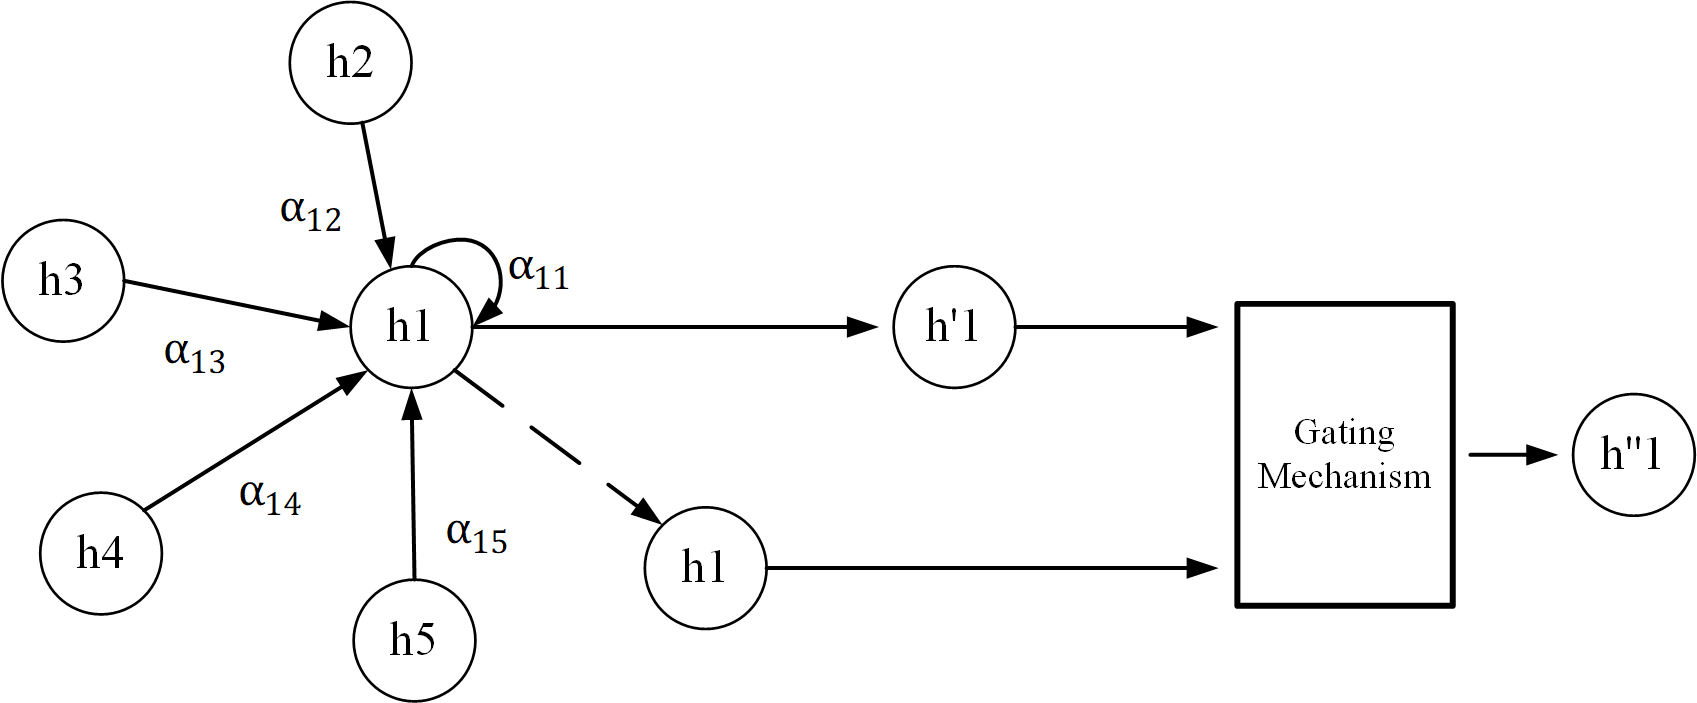
\includegraphics[width=1\textwidth]{pic/attgcn.png}
	\caption{方面级情感分析算法模型}
	\label{attgcn}
\end{figure}
节点向量为$h1$,它的邻居节点向量分别是$h2$、$h3$、$h4$、$h5$。为了选择最当前节点最重要的邻居节点,本章中采用多头注意力机制去计算,获取不同邻居节点对当前节点的权重。首先,
当前节点的向量及其邻居节点向量经过一个线性变化得到注意力机制中的q、k向量,每个向量的计算过程如公式\ref{4attQ}和公式\ref{4attK}所示。其中$W_Q$和$W_K$均是一个维度大小$d\times n$的参数矩阵。
\begin{equation}\label{4attQ}
    q = W_Qh_i, W_Q\in \mathbb{R}^{d\times n}
\end{equation}
\begin{equation}\label{4attK}
    k_i = W_Kh_i, W_K\in \mathbb{R}^{d\times n}
\end{equation}

本章计算方式中查询向量q是指当前节点向量$h1$变换后得到,而对于k向量是当前节点以及当前节点的所有邻居节点的线性变换,因此对于这些节点得到一个
$d*m$的矩阵K,其中$d$为向量维度大小,$m$是指节点个数,如图\ref{attgcn}所示,$m$为5。于是可以得到每个节点对应的注意力分数$\alpha_i$,计算公式如\ref{4attscore}所示。其中$leakyRelu$是一种激活函数。
计算方式如公式\ref{4attleakyRelu}所示,$c$是一个超参数,通常取0.001。
\begin{equation}\label{4attscore}
    \alpha_i = \frac{exp(leakyRelu(\mathbf{q}^\mathsf{T}k))}{\sum_{j}exp(leakyRelu(\mathbf{q}^\mathsf{T}k))}
\end{equation}

\begin{equation}\label{4attleakyRelu}
y_i =
\begin{cases}
x_i & \text{$x_i>=0$} \\
\frac{x_i}{c} & \text{$x_i<0$}
\end{cases}
\end{equation}

再将所有节点的向量输入一个线性变换得到v值,计算方式如公式\ref{4attV}所示,其中$W_K$是一个$d\times n$大小的参数矩阵。$tanh$为激活函数。
因此经过注意力机制更新后得到当前节点新的向量表示为$v'$,如公式\ref{4atth}所示。因为本章使用多头注意力机制,因此有多个注意力计算参与,其中
线性变换参数均有不同,因此最终该节点的向量表示应该为$h'= concat(v'_1,v'_2,...,v'_t)$,其中$t$代表$t$头注意力机制。
\begin{equation}\label{4attV}
    v_i = tanh(W_Vh_i), W_V\in \mathbb{R}^{d\times n}
\end{equation}

\begin{equation}\label{4atth}
    v' = \sum_{j}v_j* \alpha_j
\end{equation}

考虑到多层的GCN网络,每增加一层的计算,当前节点便会获取到更远邻居的信息,而远处节点的信息不一定对当前节点有用,同时还可能导致信息平滑问题,即
当层数深且图较小时,同一连通分量内的节点的表征会趋向于收敛到同一个值\citing{kipf2016semi}。这是由于一方面当前节点容易过多的吸收其他邻居节点的信息而损失了自身节点信息,
另一方面层数加深后,当前节点会获取到更广泛的其他节点信息,这就导致不同节点可能会收到相同的一组邻居节点的信息,使得信息趋于相同。已有部分工作用以解决
这种问题\citing{2018arXiv180603536X,Li_2019_ICCV}。本章采用门控机制,利用GRU中的一个更新门和一个重置门去处理这种问题。首先将GCN网络每一层中
当前节点经过注意力机制更新后的向量$h'$即如图\ref{attgcn}中的向量$h'1$和当前节点处理前的向量$h$即如图\ref{attgcn}中的向量$h1$进行拼接,得到$h_c$,如公式\ref{hconcat}所示。
\begin{equation}\label{hconcat}
    h_c = concat(h',h)
\end{equation}

之后将这个向量分别输入到更新门和重置门,计算过程如公式\ref{ztformul}和公式\ref{rtformul}所示。其中$z_t$和$r_t$分别表示更新门和重置门。$W_{zt}$、$W_{rt}$分别为
更新门和重置门的参数矩阵。$sigmoid$为激活函数,取值为0-1之间,计算如公式\ref{sigmoid}所示。
\begin{equation}\label{ztformul}
    z_t = sigmoid(W_{zt}h_c)
\end{equation}

\begin{equation}\label{rtformul}
    r_t = sigmoid(W_{rt}h_c)
\end{equation}

\begin{equation}\label{sigmoid}
    s = \frac{1}{1+exp(-x)}
\end{equation}

其中更新门用于控制前一层的节点信息被带入到当前层中的程度,更新门的值越大说明前一层的状态信息带入越多,因此得到当前节点的候选集$\tilde{h_t}$,计算如公式\ref{sht}所示。
其中$W_h$为参数矩阵,$concat$为拼接函数。
重置门控制前一层有多少信息被写入到当前的层节点信息候选集上$\tilde{h_t}$,重置门越小,前一状态的信息被写入的越少,因此可以得到最终的节点向量表示$h_t$,如公式\ref{shtt}所示。

\begin{equation}\label{sht}
    \tilde{h_t} = tanh(W_hconcat(z_t*h,h'))
\end{equation}

\begin{equation}\label{shtt}
    h_t = (1-r_t)*h'+r_t*\tilde{h_t}
\end{equation}

$h_t$即为每一层GCN的输出,经过最后一层GCN网络,将会得到一个超节点向量$e_c$和文本中的所有单词向量矩阵$E_w$,其中第i个单词的输出向量为$e_i$。

\subsection{向量融合及分类}
超节点向量$e_c$可以视作是方面词的信息向量,一段文本中对于某个方面词的情感倾向应该取决于文本中的某个词或者多个词,而方面词本身大多数仅仅是一个名词,而没有情感色彩。因此
需要通过方面词的信息从上下文中找出能代表这个方面词情感的词汇。故而本节依然采用一个多头注意力机制进行查找。通过方面词向量关注对这个词具有感情描述的其他的词汇。因此通过
注意力机制可以最终得到表示整个文本情感色彩的向量$e_a$,计算过程如公式\ref{a1},\ref{a2},\ref{a3}所示。其中$W'_q$、$W'_k$、$W'_v$均为用以线性变换的参数矩阵。
\begin{equation}\label{a1}
    a_i = \frac{(W'_qe_c)^\mathrm{T}(W'_ke_i)}{\sqrt{n}}
\end{equation}

\begin{equation}\label{a2}
    \alpha_i = \frac{a_i}{\sum_{j}exp(a_j)}
\end{equation}

\begin{equation}\label{a3}
    e_a = \sum_{j}tanh(W'_vv_j)* \alpha_j
\end{equation}

最终将超节点向量$e_c$和向量$e_a$进行拼接输入到线性变化层以及一个softmax函数得到最终输出向量,其中每一维的数值代表预测归属于某一类别标签的概率,本章算法中选择预测概率
最高的标签作为预测标签,以实现方面级情感分类任务。计算过程如公式\ref{eo},\ref{output}所示。其中$W_o$为输出层的权重矩阵,$b_o$为偏置。
\begin{equation}\label{eo}
    e_o = concat(e_c,e_a)
\end{equation}
\begin{equation}\label{output}
    O = softmax(W_oe_o+b_o)
\end{equation}

该模型利用反向传播(BP)算法进行参数更新,同时使用了Dropout防止模型过拟合。模型迭代N次,直至收敛,最终模型即可在测试集上验证分类效果,实现方面级情感分析任务。

\section{实验设置}
\subsection{数据集描述及数据处理}
本章使用方面级情感分析任务中常用的数据集,包括Twitter数据集,其由Dong等人构建而来\citing{dong-etal-2014-adaptive},以及另外三种数据集,LAP 14,Rest 14,Rest 15。
LAP 14和Rest 14来自于SemEval 2014 task 4\citing{pontiki-etal-2014-semeval},Rest 15来自于SemEval 2015 task 12\citing{pontiki-etal-2015-semeval},这四种数据集
均为英文数据集。本章分别在这四种数据集上进行验证模型及与其他模型进行对比。

\textbf{Twitter}数据集来自于Twitter上的一些关于名人、产品和公司等评论。总共有6940个文本,其中训练集包含6248段文本以及692个测试集。
该数据集共有三种类别,分别是正向情感,负面情感以及无情感倾向。以文本“i love my kindle , i really do .”为例,在这个数据集中,对应的方面词为“kindle”,
对应的标签为“1”,即正面情感。该数据集即需要根据给出的方面词,判断这个方面词在这段文本中所包含的情感色彩。

\textbf{LAP 14}数据集主要是关于电脑方面的一些评价。总共有2966个文本,其中测试集638个,2328个训练集。与twitter数据集一致,依然是正向、负面以及
无情感三种类别。以句子“it is the perfect size and speed for me”为例,其中“perfect”为方面词,其对应的标签为“1”,即正面情感,可以从单词“perfect”得出
这个结论。

\textbf{Rest 14和Rest 15}两种数据集来自于不同的年份的关于餐厅的评论。Rest 14包含4728个样本,其中共计3608个训练集以及1120个测试集。
Rest 15包含1746个样本,其中包括1204个训练集以及542个测试集,两者均与上类似为3类标签。数据集中的样本如句子“i recommend this place to everyone”为例,这个句子中给定的方面词为“place”,
从整个句子可以分析出,对于这个方面词给予的是正面评价,这从给定的标签为“1”得到验证。


\begin{table*}[htb]
	\centering
	\caption{数据集数据统计}
	
	\setlength{\tabcolsep}{0.7mm}{
		
		\begin{tabular}{c|c|c|c|c}
			\hline 
			{数据集} & {划分} & {正向}& {负向} & {无倾向}   \\
			\hline 
			\multirow{2}*{$ \text{Twitter} $}
			& 训练集 & $  1561$ & $  1560 $& $ 3127 $    \\ 
			~ & 测试集 & $   173$ & $  173 $& $ 346 $    \\ \hline
			\multirow{2}*{$ \text{LAP14} $}
			& 训练集 & $  994$ & $   870 $& $ 464 $    \\ 
			~ & 测试集 & $   341$ & $   128 $& $ 169 $    \\ \hline
			\multirow{2}*{$ \text{Rest 14} $}
			& 训练集 & $  2164$ & $  807 $& $ 637 $    \\ 
			~ & 测试集 & $   728$ & $  196 $& $ 196 $    \\ \hline
			\multirow{2}*{$ \text{Rest 15} $}
			& 训练集 & $  912$ & $  256 $& $ 36 $    \\ 
			~ & 测试集 & $   326$ & $   34 $& $ 182 $    \\ \hline
		\end{tabular}%
		\label{summaryAspect}%
	}
\end{table*}